\documentclass[conference]{IEEEtran}
\usepackage{graphicx}

% correct bad hyphenation here
\hyphenation{op-tical net-works semi-conduc-tor}


\begin{document}
%
% paper title
% can use linebreaks \\ within to get better formatting as desired
\title{Need for Suboptimal Time management in Non-ideal Shared space}


% author names and affiliations
% use a multiple column layout for up to three different
% affiliations
\author{\IEEEauthorblockN{Praveen Kumar Pendyala}
\IEEEauthorblockA{Information and Communication Engineering\\
Technische Universitat Darmstadt\\
Email: m@praveen.xyz}}

% make the title area
\maketitle


\begin{abstract}
%\boldmath
Time management is an asset and a liability. Lack of proper time management may put oneself on a depression feedback loop [1]. Time management is a melange of various aspects - scheduling tasks, execution and time line corrections, to name a few. Each of these aspects can be thought as a subproblem in our attempts to tackle the grand problem - Optimal Time Management. In addition to these subproblems, we must accept the fact that we live in a non-ideal world along with many others - shared space.  The paper deducts the need for an adaptive, suboptimal Time Management techniques taking external stimulus into consideration.
\end{abstract}


% For peer review papers, you can put extra information on the cover
% page as needed:
% \ifCLASSOPTIONpeerreview
% \begin{center} \bfseries EDICS Category: 3-BBND \end{center}
% \fi
%
% For peerreview papers, this IEEEtran command inserts a page break and
% creates the second title. It will be ignored for other modes.
\IEEEpeerreviewmaketitle


\section{Introduction}
% \IEEEPARstart
Time and Time Management are of paramount importance. This brings in an obvious urge to develop various techniques for an optimal time management technique. Starting from marking calender to a rigid time plan accounting for each hour of a day. There are a whole lot of techniques to make a basic plan, some of which will be covered in the existing literature section. One major aspect of time management is making a perfect schedule but an even more crucial part kicks in during its execution. There are several factors that could keep one from meeting their time plan. Stress, Bad planning, Lack of self control etc., which are mostly internal factors - in the sense that their correction is solely dependent on the individual. There are also external factors that could affect ones time plan - factors which the individual may not have anticipated or predicted at the time of planning.

The source of all the factors that affect time plans, broadly speaking, are a result of the fact that we live in a shared space where we are affected not only by our own actions but also by the choices of those around us and that we live in a non-ideal world where most events are probability based, not guided by any standard Uncertainty Principle, brings in more players into the equation. All these complex parameters would push any purely mathematical or conceptual approach to derive an optimal time plan into solving an NP-Hard problem [2]. One has to live with a suboptimal time plan for a given situation, iterate it based on their needs and arrive at an acceptable compromise between an ideal and executable plan.

The following contents of the paper are divided into four sections. Section II. Existing literature would focus on some of the existing techniques for Time management. Followed by Section III. Execution and Evaluation which is completely spanned by a case study where the subject employs an adaptive time management technique for their day to day activity for two fortnights. We will then conclude with Section IV. Conclusions, where would be highlighting the key aspects of our argument and how we derived or observed them in the case of the test subject.

\section{Existing literature}
There is plethora of research related to Time Management (TM) techniques and surveys depicting the outcomes of adopting or otherwise of a TM technique. [3], [4] and [5] centered their work around the impact of TM in an academic context, backing their claims through surveys with varying size of sample space and interpretations but similar outcomes. Time Management behaviors may have beneficial effects on tensions and job satisfaction but not on job performance. Contrary to popular claims, time management training was not found to be effective [6]. This controverts the hypothesis and findings of [7] and [8].

\begin{figure}[hb]
  \centering
  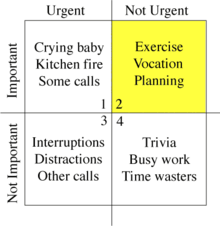
\includegraphics[width=2.2in]{eisenhower}
  \caption[]
   {A basic "Eisenhower box" to help evaluate urgency and importance.}
\end{figure}

Some of the very common time management methodologies are Pareto analysis, ABC analysis and The Eisenhower Method. The central idea of Pareto analysis is that 80\% of tasks can be completed in 20\% of the disposable time - The 80-20-rule to increase productivity [12]. ABC analysis is often used in business management for categorization of large data into groups [11]. These groups are often marked A -- Tasks that are perceived as being urgent and important, B -- Tasks that are important but not urgent, and C -- Tasks that are neither urgent nor important. Each group is then rank-ordered by priority. Last in our list, The Eisenhower Method, uses the Eisenhower Decision Principle through which, all tasks are evaluated using the criteria important/unimportant and urgent/not urgent, and then placed in according quadrants in an Eisenhower Matrix as shown in figure 1.


The common shortcoming in all these literatures is their failure to account that test subjects could be influenced by a plethora of external and internal factors. All these influencing factors, broadly speaking, are a result of Non-idealistic behavior and shortcomings of the test subjects and negative, intended or unintended, influence from peers, colleagues and other indirect players on test subject's attempts in keeping up with their schedule. Attempts have been made to evaluate the extent of influence by a common factor, tendency of procrastination, on the effective execution of ones time plan [9], [10].


\section{Execution and Evaluation}
We analyzed the day-to-day life executions of a test subject and how they divulge from their expected time plan. A qualitative note on the external factors causing the time-line diversion is also provided corresponding to each diversion.


\begin{figure}[hb]
  \centering
	  \begin{tabular}{ | l | c | }
		\hline
		\textbf{Activity type} 	& \textbf{Time spent per day} 	\\ \hline
		Sleep					& 	8 Hours						\\ \hline
		Job						& 	5 Hours						\\ \hline
		Lectures				& 	3 Hours						\\ \hline
		Learning				& 	3 Hours						\\ \hline
		Leisure					& 	5 Hours						\\ \hline
	  \end{tabular} 
  \caption[]
   {Static reference time line plan made by the test subject}
\end{figure}

We began the experiment by making a static time plan for the test subject as shown in figure 2. This serves as a reference while the actual time spent on a given activity per day, almost always, is different from the planned schedule. The differences are mostly consistent over span of few days which tells us that the external factors causing this offset are stable influences coming from the shared space concept depicted earlier. To shed some more light on this behavior, we calculated the time spent per activity in a period of one week and tabulated the values for four weeks as shown in figure 3. 

\begin{figure}[hb]
  \centering
  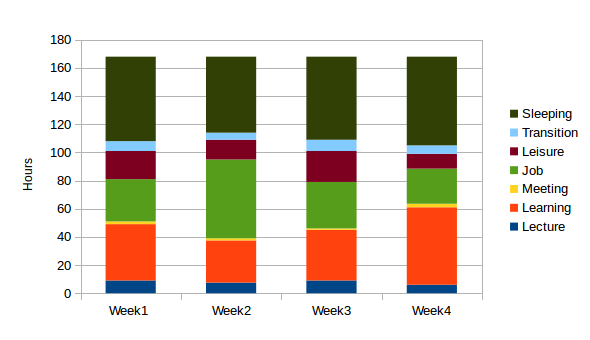
\includegraphics[width=3.7in]{bar}
  \caption[]
   {Hours spent per activity in a week for a period of four weeks}
\end{figure}

An interesting observation here is that only a certain type of activity times vary significantly across weeks while others are nearly stable. The relatively stable time share is taken on every week by Sleep, Transition and Lectures with the significantly varying ones being Leisure, Job and Learning. We can qualitatively identify the factors causing these changes in a given week compared to the average or planned static time line. The external factors that influence an increased shared in Job activity are work related deadlines, presentations and goals. The ones that root for a share increase of Academic activities - Learning and Lectures being Lab work / demos, Exams and other academic deadlines. We can also notice a dip in Lectures timeshare in week 4 where the subject is loaded by other forms of academic activity like project or lab deadlines. 

The variance in activity time share can be observed better in figure 4. where we identified two extreme weeks - one involving a greater share on Academic activity and the later with a greater share on Work activity, and compared it with an average time share of each activity over the whole period of four weeks. Innermost ring represents learning dominated week, middle ring for average over four weeks, outermost ring represents job dominated week. The arc angle covered by the stable activities is nearly same across all the rings while the unstable activities showing an angular variance of 10-15 percent. The not so high, yet not negligible, variance in dynamic activity timeshares indicate that the concept of a single static reference is bad and good at the same time. This leads us to believe that influences from external factors are inevitable and test subject has employed subjective ways to cope up with them and follow a suboptimal time management scheme.

\begin{figure}[hb]
  \centering
  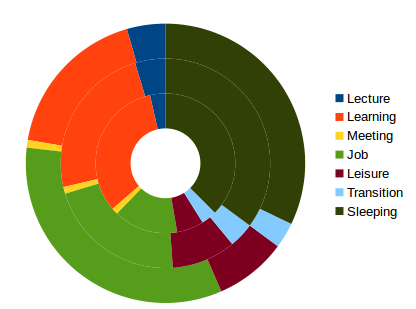
\includegraphics[width=3.7in]{donut}
  \caption[]
   {Concentric rings pie chart depicting the time share of each activity in a week over 3 different week samples. Innermost ring represents learning dominated week, middle ring for average over four weeks, outermost ring represents job dominated week}
\end{figure}


\section{Conclusions}
We presented the existing literature on Time management, majority of which dealt with assumptions of static time management. We then followed on to listing factors - external and internal, that affect such a scheme and established the need for adaptive or dynamic planning. We presented a case study on Test subject who employed a static time plan to start with and displayed significant deviations from the plan on day-to-day basis. We observed patterns in this deviations and provided a qualitative analysis of plausible external factors that may have caused the deviations for each type of activity over one week. In conclusion, we established that we are affected by various factors in following a static time line and that majority of these stimulus are a direct implication of the fact that we live in a non-ideal world of probabilities along with others. Thus one may employ a static time plan which may be used as a reference and should be willing to adapt to the changes.

% use section* for acknowledgement
\section*{Acknowledgment}
The author would like to extend his gratitude to the Telecooperation Group of TU Darmstadt for providing the required tools and resources, which form the basis for Test Subject Data collection and served as seed for this paper.


% trigger a \newpage just before the given reference
% number - used to balance the columns on the last page
% adjust value as needed - may need to be readjusted if
% the document is modified later
%\IEEEtriggeratref{8}
% The "triggered" command can be changed if desired:
%\IEEEtriggercmd{\enlargethispage{-5in}}

% references section

\begin{thebibliography}{1}

\bibitem{IEEEhowto:}
\emph{Yoga Journal}, \relax May-Jun 1976, pp. 17.

\bibitem{IEEEhowto:}
Aaronson, Scott. \emph{"NP-complete problems and physical reality."} ACM Sigact News 36.1, 2005, pp. 30-52.

\bibitem{IEEEhowto:}
Britton, Bruce K., and Abraham Tesser. \emph{"Effects of time-management practices on college grades."} Journal of educational psychology 83.3 (1991): 405.

\bibitem{IEEEhowto:}
Macan, Therese H., et al. \emph{"College students' time management: Correlations with academic performance and stress."} Journal of educational psychology 82.4 (1990): 760.

\bibitem{IEEEhowto:}
Misra, Ranjita, and Michelle McKean. \emph{"COLLEGE STUDENTS'ACADEMIC STRESS AND ITS RELATION TO THEIR ANXIETY, TIME MANAGEMENT, AND LEISURE SATISFACTION."} American Journal of Health Studies 16.1 (2000): 41-51.

\bibitem{IEEEhowto:}
Macan, Therese Hoff. \emph{"Time management: Test of a process model."} Journal of applied psychology 79.3 (1994): 381.

\bibitem{IEEEhowto:}
Adams, Gary A., and Steve M. Jex. \emph{"Relationships between time management, control, work–family conflict, and strain."} Journal of Occupational Health Psychology 4.1 (1999): 72.

\bibitem{IEEEhowto:}
Waterworth, Susan. \emph{"Time management strategies in nursing practice."} Journal of Advanced Nursing 43.5 (2003): 432-440.

\bibitem{IEEEhowto:}
Lay, Clarry H., and Henri C. Schouwenburg. \emph{"Trait procrastination, time management, and academic behavior."} Journal of Social Behavior and Personality (1993).

\bibitem{IEEEhowto:}
Gafni, Ruti, and Nitza Geri. \emph{"Time management: Procrastination tendency in individual and collaborative tasks."} Interdisciplinary Journal of Information, Knowledge, and Management 5 (2010): 115-125.

\bibitem{IEEEhowto:}
Lakein, Alan. How to Get Control of Your Time and Your Life. New York: P.H. Wyden (1973)

\bibitem{IEEEhowto:}
Timothy Ferris. \emph{"The 4-Hour Workweek."} Crown Publishing Group (2007)

\bibitem{IEEEhowto:}
McKay, Brett and Kate. \emph{"The Eisenhower Decision Matrix: How to Distinguish Between Urgent and Important Tasks and Make Real Progress in Your Life."} A Man's Life, Personal Development. (October 23, 2013)


\end{thebibliography}




% that's all folks
\end{document}


